\hypertarget{contributions}{%
\subsection{Contributions}\label{contributions}}

This material is this chapter expands on work presented in

\autocite{hodsonOnedimensionalLongRangeFalikovKimball2021} \href{https://link.aps.org/doi/10.1103/PhysRevB.104.045116}{One-dimensional long-range Falikov-Kimball model: Thermal phase transition and disorder-free localization}, Hodson, T. and Willsher, J. and Knolle, J., Phys. Rev.~B, \textbf{104}, 4, 2021,

Johannes had the initial idea to use a long range Ising term to stablise order in a one dimension Falikov-Kimball model. Josef developed a proof of concept during a summer project at Imperial. The three of us brought the project to fruition.

\hypertarget{chapter-summary}{%
\subsection{Chapter Summary}\label{chapter-summary}}

To evaluate thermodynamic averages we perform a classical Markov Chain Monte Carlo random walk over the space of ionic configurations, at each step diagonalising the effective electronic Hamiltonian \textcite{maskaThermodynamicsTwodimensionalFalicovKimball2006}\}. Using a binder-cumulant method \autocite{binderFiniteSizeScaling1981,musialMonteCarloSimulations2002}, we demonstrate the model has a finite temperature phase transition when the interaction is sufficiently long ranged. We then estimate the density of states and the inverse participation ratio as a function of energy to diagnose localisation properties. We show preliminary results that the in-gap states induced at finite temperature are localised while the states in the unperturbed bands remain extended, evidence for a mobility edge.

Despite its simplicity, the FK model has a rich phase diagram in \(D \geq 2\) dimensions. For example, it shows an interaction-induced gap opening even at high temperatures, similar to the corresponding Hubbard Model~\autocite{brandtThermodynamicsCorrelationFunctions1989}. In 1D, the ground state phenomenology as a function of filling can be rich~\autocite{gruberGroundStatesSpinless1990} but the system is disordered for all \(T > 0\)~\autocite{kennedyItinerantElectronModel1986}. Moreover, the model has been a test-bed for many-body methods, interest took off when an exact DMFT solution in the infinite dimensional case was found~\autocite{antipovCriticalExponentsStrongly2014,ribicNonlocalCorrelationsSpectral2016,freericksExactDynamicalMeanfield2003,herrmannNonequilibriumDynamicalCluster2016}.

\hypertarget{the-model}{%
\section{The Model}\label{the-model}}

The Falikov-Kimball (FK) model \[\begin{aligned}
H_{\mathrm{FK}} = & \;U \sum_{i} S_i\;(c^\dagger_{i}c_{i} - \tfrac{1}{2}) -\;t \sum_{i} (c^\dagger_{i}c_{i+1} + \textit{h.c.)}\\ 
\end{aligned}\] is one of the simplest models of the correlated electron problem. It captures the essence of the interaction between itinerant \(c_i\) and localized electrons, equivalent to a model of hopping fermions coupled to a classical Ising field \(S_i = \pm 1\). It was originally introduced to explain the metal-insulator transition in f-electron systems but in its long history it has been interpreted variously as a model of electrons and ions, binary alloys or of crystal formation~\autocite{hubbardj.ElectronCorrelationsNarrow1963,falicovSimpleModelSemiconductorMetal1969,gruberFalicovKimballModelReview1996,gruberFalicovKimballModel2006}.

One can look to the references above to see why one might write the FK Model down directly. Here, in order to motivate the connection to exactly solvable models, I will explain how the Falikov-Kimball model is a particular limit of the Hubbard Model \[\begin{aligned}
H_{\mathrm{H}} = & \;U \sum_{i} n_{i\downarrow} n_{i\uparrow} -\;t \sum_{i\alpha} c^\dagger_{i,\alpha}c_{i+1,\alpha} + \mu \sum_{i\alpha} n_{i\alpha} + \textit{h.c.} \\ 
\end{aligned}\]

The Hubbard model is one of interacting spin-\(\tfrac{1}{2}\) electrons hopping on a lattice. It has been the subject of intense study for many years but, as an interacting many body quantum system, analytic handles on it are few and far between. There is still much we don't know about the Hubbard Model.

Usually the Hubbard model is written with equal hopping for the two spins states \(t_\uparrow = t_\downarrow\) have included a spin dependent hopping term \(t_\alpha\)

\begin{Shaded}
\begin{Highlighting}[]

\end{Highlighting}
\end{Shaded}

\hypertarget{localisation}{%
\subsection{Localisation}\label{localisation}}

The discovery of localisation in quantum systems surprising at the time given the seeming ubiquity of extended Bloch states. Later, when thermalisation in quantum systems gained interest, localisation phenomena again stood out as counterexamples to the eigenstate thermalisation hypothesis \autocite{abaninRecentProgressManybody2017,srednickiChaosQuantumThermalization1994}, allowing quantum systems to avoid to retain memory of their initial conditions in the face of thermal noise.

The simplest and first discovered kind is Anderson localisation, first studied in 1958 \autocite{andersonAbsenceDiffusionCertain1958} in the context of non-interacting fermions subject to a static or quenched disorder potential \(V_j\) drawn uniformly from the interval \([-W,W]\)

\[
H = -t\sum_{\langle jk \rangle} c^\daggerger_j c_k + \sum_j V_j c_j^\daggerger c_j
\]

this model exhibits exponentially localised eigenfunctions \(\psi(x) = f(x) e^{-x/\lambda}\) which cannot contribute to transport processes. Initially it was thought that in one dimensional disordered models, all states would be localised, however it was later shown that in the presence of correlated disorder, bands of extended states can exist \autocite{izrailevLocalizationMobilityEdge1999,croyAndersonLocalization1D2011,izrailevAnomalousLocalizationLowDimensional2012}.

Later localisation was found in interacting many-body systems with quenched disorder:

\[
H = -t\sum_{\langle jk \rangle} c^\daggerger_j c_k + \sum_j V_j c_j^\daggerger c_j + U\sum_{jk} n_j n_k
\]

where the number operators \(n_j = c^\dagger_j c_j\). Here, in contrast to the Anderson model, localisation phenomena can be proven robust to weak perturbations of the Hamiltonian. This is called many-body localisation (MBL) \autocite{imbrieManyBodyLocalizationQuantum2016}.

Both MBL and Anderson localisation depend crucially on the presence of quenched disorder. This has led to ongoing interest in the possibility of disorder-free localisation, in which the disorder necessary to generate localisation is generated entirely from the dynamics of the model. This contracts with typical models of disordered systems in which disorder is explicielty introduced into the Hamilton or the initial state.

The concept of disorder-free localisation was first proposed in the context of Helium mixtures \autocite{kagan1984localization} and then extended to heavy-light mixtures in which multiple species with large mass ratios interact. The idea is that the heavier particles act as an effective disorder potential for the lighter ones, inducing localisation. Two such models \autocite{yaoQuasiManyBodyLocalizationTranslationInvariant2016,schiulazDynamicsManybodyLocalized2015} instead find that the models thermalise exponentially slowly in system size, which Ref. \autocite{yaoQuasiManyBodyLocalizationTranslationInvariant2016} dubs Quasi-MBL.

True disorder-free localisation does occur in exactly solveable models with extensively many conserved quantities \autocite{smithDisorderFreeLocalization2017}. As conserved quantites have no time dynamics this can be thought of as taking the separation of timescales to the infinite limit.

\hypertarget{the-falikov-kimball-model}{%
\subsubsection{The Falikov Kimball Model}\label{the-falikov-kimball-model}}

In the Falikov Kimball (FK) model spinless fermions \(c_{i\uparrow}\) are coupled via a repulsive on-site interaction to a classical degree of freedom \(n_{i\downarrow}\).

\[\begin{aligned}
H &= -t \sum_{<ij>} c^\daggerger_{i\uparrow}c_{j\uparrow} + U \sum_{i} (n_{i \uparrow} - 1/2)( n_{i\downarrow} - 1/2) \\
       & - \mu \sum_i \left( n_{i \uparrow} + n_{i \downarrow} \right) + \sum_{ij} V_{ij} (n_{i\downarrow} - 1/2)(n_{j\downarrow} - 1/2) 
\end{aligned}\] \textbf{replace with hamiltonian from the paper}

This notation emphasises that this can also be thought of as an asymmetric Hubbard model in which the spin down electrons cannot hop and are subject to an additional long range potential. However, to avoid the confusion of talking about two distinct species of spinless electrons we will use a different interpretation and refer to the classical degrees of freedom as the ``ionic sector'' and the quantum degrees of freedom as the ``electronic sector''. The final term that induces interactions between the classical particles has been added by us to stabilise the formation of an ordered phase in 1D. The classical variables commute with the Hamiltonian \([H, n_{i\downarrow}] = 0\) so like the lattice gauge model in Ref \autocite{smithDisorderFreeLocalization2017} the FK model has extensively many conserved quantities which can act as an effective disorder potential for the electronic sector.

Due to Pauli exclusion, the maximum filling occurs when one of each species occupies each lattice site such that \(\sum_i (n_{i\downarrow} + n_{i\uparrow} )/ N = 2\). Here we focus on the half filled case which also displays particle-hole symmetry (see later).

\hypertarget{falikov-kimball-and-hubbard-models}{%
\subsection{Falikov Kimball and Hubbard models}\label{falikov-kimball-and-hubbard-models}}

We will first introduce the standard Hubbard and Falikov-Kimball (FK) models then look at some of their properties. We'll then cover why the Falikov-Kimball model represents an interesting system in which to study disorder free localisation.

\hypertarget{hubbard-model}{%
\subsubsection{Hubbard model}\label{hubbard-model}}

The Hubbard model gives a very simple setting in which to study interacting, itinerant electrons. It is a tight binding model of spin half electrons with finite bandwidth \(t\) and a repulsive on-site interaction \(U > 0\).

\[
    H = -\sum_{<ij>,\sigma} t_{\sigma} c^\dagger_{i\sigma}c_{j\sigma} + U \sum_{i} (n_{i \uparrow} - 1/2)( n_{i\downarrow} - 1/2) - \mu \sum_i \left( n_{i \uparrow} + n_{i \downarrow} \right)
\]

in standard notation. The standard Hubbard model corresponds to the case \(t_{\uparrow} = t_{\downarrow}\). Here we have used the particle-hole symmetric version of the interaction term, which is more often given as \(n_{i \uparrow} n_{i\downarrow}\). The difference just amounts to a redefinition of the chemical potential.

Hubbard originally used the model at half filling \(\mu = 0\) to explain the Mott metal-insulator (MI) transition, however it has seen applications to high-temperature superconductivity and become target for cold-atom optical trap experiments. \autocite{HubbardModelHalf2013,greiner_quantum_2002,jordens_mott_2008}. While simple, only a few analytic results exist, namely the Bethe ansatz \autocite{liebAbsenceMottTransition1968} which proves the absence of even a zero temperature phase transition in the 1D model and Nagaoka's theorem \autocite{nagaokaFerromagnetismNarrowAlmost1966} which proves that the three dimensional model has a ferromagnetic ground state in the vicinity of half filling.

\hypertarget{falikov-kimball-model}{%
\subsubsection{Falikov-Kimball model}\label{falikov-kimball-model}}

\begin{figure}
  \centering
    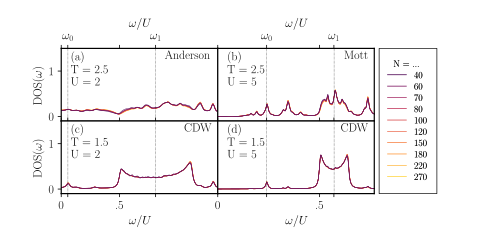
\includegraphics[width=\textwidth]{figs/DOS}
  \caption{Density of states for the Anderson model with (a) no potential, (b) a charge density wave (CDW) potential $\vec{h} = (0,1,0,1...)$, (c) a disordered CDW potential each site has an uncorrelated $2\%$ chance of deviating from the CDW background. Hopping and potential terms both have unit magnitude.}
  \label{fig:fk_dos}
\end{figure}

The Falikov-Kimball model corresponds to the case \(t_{\downarrow} = 0\). It can be interpreted as two coupled spinless electron bands with infinite mass ratio. An itinerant light species with creation operator \(c^\dagger_{i\uparrow}\) coupled to an infinitely heavy, immobile species with density operator \(n_{i\downarrow}\). These are often called c and f electrons or electrons and ions. The model was first introduced by Hubbard in 1963 as a model of interacting localised and de-localised electron bands and gained its name from Falikov and Kimball's use of it to study the MI transition in rare-earth materials \autocite{hubbardj.ElectronCorrelationsNarrow1963,falicov_simple_1969}.

Here we will use refer to the light spinless species as \emph{electrons} with creation operator \(c^\dagger_{i}\) and the heavy species as \emph{ions} with density operator \(n_i\). When the the density operator of the electrons is needed I'll always use \(c^\dagger_{i}c_{i}\). We also set \(t = 1\).

\[
    H_{\mathrm{FK}} = -\sum_{<ij>} c^\dagger_{i}c_{j} + U \sum_{i} (c^\dagger_{i}c_{i} - 1/2)( n_i - 1/2) - \mu \sum_i \left(c^\dagger_{i}c_{i} + n_{i}\right)
\] \% \#\#\# Particle-Hole Symmetry The Hubbard and FK models on a bipartite lattice have particle-hole (PH) symmetry \(P^\dagger H P = - H\), accordingly they have symmetric energy spectra. The associated symmetry operator \(P\) exchanges creation and annihilation operators along with a sign change between the two sublattices.

\[ d^\dagger_{i\sigma} = (-1)^i c_{i\sigma}\] \% The entirely filled state \(\ket{\Omega} = \sum_{j\rho} c^\dagger_{j\rho} \ket{0}\) becomes the new vacuum state: \[d_{i\sigma} \ket{\Omega} = (-1)^i c^\dagger_{i\sigma} \sum_{j\rho} c^\dagger_{j\rho} \ket{0} = 0\] \% The number operator \(n_{i\sigma} = 0,1\) counts holes rather than particles: \[ d^\dagger_{i\sigma} d_{i \sigma} = c_{i\sigma} c^\dagger_{i\sigma} = 1 - c^\dagger_{i\sigma} c_{i\sigma}\] \% With the last equality following from the fermionic commutation relations. In the case of nearest neighbour hopping on a bipartite lattice this transformation also leaves the hopping term unchanged: \[ d^\dagger_{i\sigma} d_{j \sigma} = (-1)^{i+j} c_{i\sigma} c^\dagger_{j\sigma} = c^\dagger_{i\sigma} c_{j\sigma} \] \% Since when \(i\) and \(j\) label sites on separate sublattices, \((-1)^{i-j} = -1\) and this is absorbed into rearranging the operators via their anti-commutator.

Defining the particle density \(\rho\) as the number of fermions per site: \[
    \rho = \frac{1}{N} \sum_i \left( n_{i \uparrow} + n_{i \downarrow} \right)
\] \% The PH symmetry maps the Hamiltonian to itself with the sign of the chemical potential reversed and the density is inverted about half filling: \[ \text{PH} : H(t, U, \mu) \rightarrow H(t, U, -\mu) \] \[ \rho \rightarrow 2 - \rho \] \% The Hamiltonian is symmetric under PH at \(\mu = 0\) and so must all the observables, hence half filling \(\rho = 1\) occurs here. This symmetry and known observable acts as a useful test for the numerical calculations.

\hypertarget{thermodynamics-of-the-fk-model}{%
\subsubsection{Thermodynamics of the FK model}\label{thermodynamics-of-the-fk-model}}

\textbackslash begin\{figure\} \centering 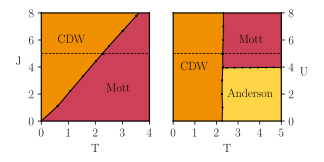
\includegraphics[width=0.8\textwidth]{figs/phase_diagram}

\caption{Phases of the 2D Falikov Kimball Model, showing the ordered charge density wave phase at low temperatures and the interaction mediated transition between Anderson localisation and Mott insulating phases in the disordered phase. [@andersonAbsenceDiffusionCertain1958]}

\} \label{fig:FK_phase_diagram} \textbackslash end\{figure\}

At half filling and in dimensions greater than one, the FK model exhibits a phase transition at some \(U\) dependent critical temperature \(T_c(U)\) to a low temperature charge density wave state in which the ions occupy one of the two sublattices A and B \autocite{maskaThermodynamicsTwodimensionalFalicovKimball2006}. The order parameter is the square of the staggered magnetisation: \[
M = \sum_{i \in A} n_i - \sum_{i \in B} n_i
\] \% In the disordered phase Ref. \autocite{andersonAbsenceDiffusionCertain1958} identifies an interplay between Anderson localisation at weak interaction and a Mott insulator phase in the strongly interacting regime.

In the one dimensional FK model, however, Peierls' argument \autocite{peierlsIsingModelFerromagnetism1936,kennedyItinerantElectronModel1986} and the Bethe ansatz \autocite{liebAbsenceMottTransition1968} make it clear that there is no ordered CDW phase. Peierls' argument is that one should consider the difference in free energy \(\Delta F = \Delta E - T\Delta S\) between an ordered state and a state with single domain wall in the order parameter. In the Ising model this would be having the spins pointing up in one part of the model and down in the other, for a CDW phase it means having the ions occupy the A sublattice in one part and the B sublattice in the other.

Short range interactions will produce a constant energy penalty for such a domain wall that does not scale with system size while in 1D there are \(L\) such states so the domain wall is associated with entropy \(S \propto \ln L\) which dominates in the thermodynamic limit. The slow logarithmic scaling suggests we should be wary of finite size scaling effects.

One dimensional systems are more amenable to numerical and experimental study so we add long range staggered interactions to bring back the ordered phase:

\[ H_{\textrm{int}} = 4J \sum_{ij} \frac{(-1)^{|i-j|}}{ |i - j|^{\alpha} } (n_i - 1/2) (n_j - 1/2) = J \sum_{ij} |i - j|^{-\alpha} \tau_i \tau_j\] \% at half-filling the modified Hamiltonian is then: \[
    H_{\mathrm{FK}}^* &= -\sum_{<ij>} c^\dagger_{i}c_{j} + U \sum_{i} (c^\dagger_{i}c_{i} - 1/2)( n_i - 1/2) \\
    &+ 4J \sum_{ij} \frac{(-1)^{|i-j|}}{ |i - j|^{\alpha} } (n_i - 1/2) (n_j - 1/2)  \\
    &= -\sum_{<ij>} c^\dagger_{i}c_{j} + 2U \sum_{i} (-1)^i (c^\dagger_{i}c_{i} - 1/2)\tau_i + J \sum_{ij} |i - j|^{-\alpha} \tau_i \tau_j  \\
\] \% The form of this interaction comes from interpreting the f-electrons as a classical Ising chain using a staggered mapping \(\tau_i = (-1)^i (2n_i^ f - 1)\) so that ferromagnetic order in the \(\tau_i\) variables corresponds to a CDW state in the \(n_i^f\) variables. It also preserves the particle hole symmetry because for the ions the PH transformation corresponds to \(n_i \rightarrow 1 - n_i\). When \(U = 0\) the model decouples into a long ranged Ising model and free fermions.

\hypertarget{long-ranged-ising-model}{%
\subsection{Long Ranged Ising model}\label{long-ranged-ising-model}}

Our extension to the FK model could now be though of as spinless fermions coupled to a long range Ising (LRI) model. The LRI model has been extensively studied and its behaviour may be bear relation to the behaviour of our modified FK model.

\[H_{\mathrm{LRI}} = \sum_{ij} J(\abs{i-j}) \tau_i \tau_j = J \sum_{i\neq j} |i - j|^{-\alpha} \tau_i \tau_j\] \% Rigorous renormalisation group arguments show that the LRI model has an ordered phase in 1D for \$1 \textless{} \alpha \textless{} 2 \$ \autocite{dysonExistencePhasetransitionOnedimensional1969}. Peierls' argument can be extended \autocite{thoulessLongRangeOrderOneDimensional1969} to provide intuition for why this is the case. Again considering the energy difference between the ordered state \(\ket{\ldots\uparrow\uparrow\uparrow\uparrow\ldots}\) and a domain wall state \(\ket{\ldots\uparrow\uparrow\downarrow\downarrow\ldots}\). In the case of the LRI model, careful counting shows that this energy penalty is: \[\Delta E \propto \sum_{n=1}^{\infty} n J(n)\] \% because each interaction between spins separated across the domain by a bond length \(n\) can be drawn between \(n\) equivalent pairs of sites. Ruelle proved rigorously for a very general class of 1D systems, that if \(\Delta E\) or its many-body generalisation converges in the thermodynamic limit then the free energy is analytic \autocite{ruelleStatisticalMechanicsOnedimensional1968}. This rules out a finite order phase transition, though not one of the Kosterlitz-Thouless type. Dyson also proves this though with a slightly different condition on \(J(n)\) \autocite{dysonExistencePhasetransitionOnedimensional1969}.

With a power law form for \(J(n)\), there are three cases to consider:

\begin{center}
    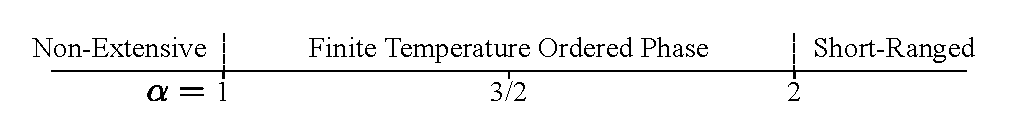
\includegraphics[width=\textwidth]{figs/alpha_diagram}
\end{center}

\begin{enumerate}
\def\labelenumi{\arabic{enumi}.}
\tightlist
\item
  \$ \alpha = 0\$ For infinite range interactions the Ising model is exactly solveable and mean field theory is exact \autocite{lipkinValidityManybodyApproximation1965}.
\item
  \$ \alpha \le 1\$ For slowly decaying interactions \(\sum_n J(n)\) does not converge so the Hamiltonian is non-extensive, a case which won't be further considered here.
\item
  \$ 1 \textless{} \alpha \textless{} 2 \$ A phase transition to an ordered state at a finite temperature.
\item
  \$ \alpha = 2 \$ The energy of domain walls diverges logarithmically, and this turns out to be a Kostelitz-Thouless transition \autocite{thoulessLongRangeOrderOneDimensional1969}.
\item
  \$ 2 \textless{} \alpha \$ For quickly decaying interactions, domain walls have a finite energy penalty, hence Peirels' argument holds and there is no phase transition.
\end{enumerate}

\hypertarget{thermodynamics}{%
\subsubsection{Thermodynamics}\label{thermodynamics}}

On bipartite lattices in dimensions 2 and above the FK model exhibits a finite temperature phase transition to an ordered charge density wave (CDW) phase \autocite{maskaThermodynamicsTwodimensionalFalicovKimball2006}. In this phase, the ions are confined to one of the two sublattices, breaking the \(\mathbb{Z}_2\) symmetry.

In 1D, however, Periel's argument \autocite{peierlsIsingModelFerromagnetism1936,kennedyItinerantElectronModel1986} states that domain walls only introduce a constant energy penalty into the free energy while bringing a entropic contribution logarithmic in system size. Hence the 1D model does not have a finite temperature phase transition. However 1D systems are much easier to study numerically and admit simpler realisations experimentally. We therefore introduce a long range coupling between the ions in order to stabilise a CDW phase in 1D. This leads to a disordered system that is gaped by the CDW background but with correlated fluctuations leading to a disorder-free correlation induced mobility edge in one dimension.

\begin{figure}
\hypertarget{fig:binder}{%
\centering
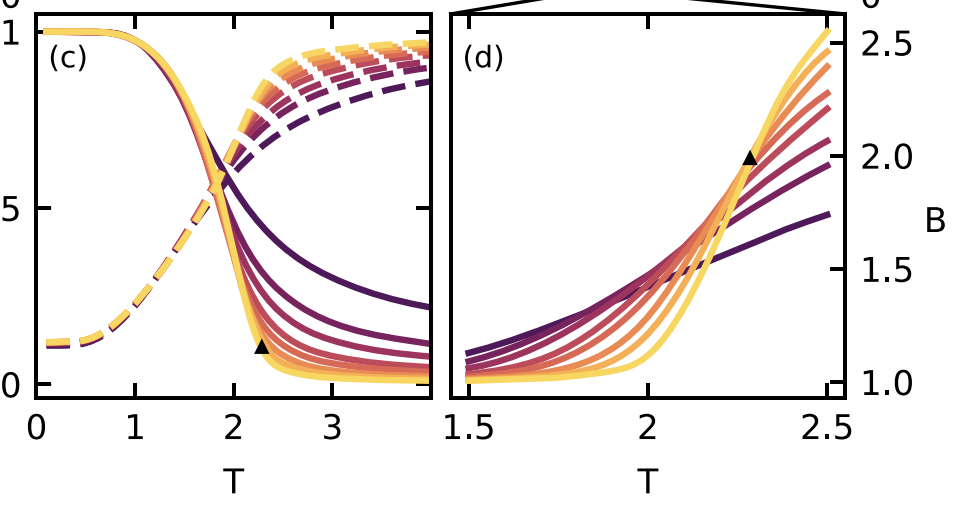
\includegraphics[width=1\textwidth,height=\textheight]{figure_code/fk_chapter/binder.png}
\caption[no title]{Hello I am the figure caption!}\label{fig:binder}
}
\end{figure}

Macro definitions in this cell \[
\newcommand{\expval}[1]{\langle #1 \rangle}
\newcommand{\ket}[1]{|#1\rangle}
\newcommand{\bra}[1]{\langle#1|}
\newcommand{\op}[2]{|#1\rangle \langle#2|}
\]

\[
\expval{O}, \op{\alpha}{\beta}, \ket{\psi}
\]

\hypertarget{localisation-1}{%
\subsection{Localisation}\label{localisation-1}}

\hypertarget{thermalisation}{%
\subsubsection{Thermalisation}\label{thermalisation}}

Isolated classical systems generally thermalise if they are large enough. Since classical dynamics is the limit of some underlying quantum dynamics, it seems reasonable to suggest that isolated quantum systems also thermalise in some related sense. However it is not immediately obvious what thermalisation should mean in a quantum setting where the presence of unitary time dynamics implies full information about a system's initial state is always preserved.

A potential solution lies in the eigenstate thermalisation hypothesis. It states that if a system thermalises, then we can isolate small patches of a larger system, trace everyhing else out, and get a thermal density matrix.

Following Ref. \autocite{abaninRecentProgressManybody2017}, consider the time evolution of a local operator \(\hat{O}\) \[ \expval{\hat{O}}{\psi(t)} = \sum_{\alpha \beta} C^*_\alpha C_\beta e^{i(E_\alpha - E_\beta)} O_{\alpha \beta}\]

Where \(C_\alpha\) are determined by the initial state and \(O_{\alpha \beta} = \expval{\alpha | \hat{O} | \beta}\) are the matrix elements of \(\hat{O}\) with respect to the energy eigenstates. Srednicki \autocite{srednickiChaosQuantumThermalization1994} introduced the ansatz that for local operators:

\[O_{\alpha \beta} = O(E)\delta_{\alpha\beta} + e^{-S(E)/2} f(E,\omega) R_{\alpha\beta}\]

with \(E = (E_\alpha + E_\beta)\), \(\omega = (E_\alpha - E_\beta)\) and \(R_{\alpha\beta}\) are sampled from some distribution with zero mean and unit variance. The first term asserts that the diagonal elements are given by the thermal expectation value \(O(E) = Tr[e^{-\beta \hat{H}} \hat{O}]/\mathcal{Z}\) with \(\beta\) an effective temperature defined by equating the energy to the expectation of the Hamiltonian at that temperature \(E = Tr[H e^{-\beta \hat{H}}/\mathcal{Z}]\).

The second term deals with thermodynamic fluctuations scaled by the entropy \(S(E) = -Tr(\rho \log \rho)\) where \(\rho = e^{-\beta \hat{H}}\) and \(\mathcal{Z} = Tr[e^{-\beta \hat{H}}]\).

With this ansatz the long time average of the observable becomes equal to the thermal expectations with fluctuations suppressed by the entropic term \(e^{-S(E)}\) and the rapidly varying phase factors \(e^{i(E_\alpha - E_\beta)}\). This statement of the ETH has verified for the quantum hard sphere model \autocite{srednickiChaosQuantumThermalization1994} and numerically for other models \autocite{khatamiFluctuationDissipationTheoremIsolated2013,dalessioQuantumChaosEigenstate2016}.

An alternate view on ETH is the statement that in thermalising systems individual eigenstates look thermal when viewed locally. Take a eigenstate \(|\alpha\rangle\) with energy \(E_\alpha\) and as before define an effective temperature with \(E_\alpha = Tr[H e^{-\beta \hat{H}}/\mathcal{Z}]\). This statement of the ETH says that if we partition the system into subsystems A and B with a limit taken as B becomes very large, B will act as a heat bath for A. Specifically the reduced density matrix \(\rho_A = Tr_B \op{\alpha}{\alpha}\) is equal to the thermal density matrix:

\[\rho_A = Tr_B |\alpha\rangle \langle \alpha| = \mathcal{Z}^{-1} Tr_B [e^{-\beta \hat{H}}] \]

Intuitively, for thermalisation to happen, the degrees of freedom must be sufficiently well coupled that energy transport occurs. This condition is broken by systems with localised states so a lack of thermalisation is often used as a diagnostic tool for localisation.

\hypertarget{anderson-localisation}{%
\subsubsection{Anderson Localisation}\label{anderson-localisation}}

Localisation was first studied by Anderson in 1958 \textcite{andersonAbsenceDiffusionCertain1958} in the context of non-interacting fermions subject to a static or quenched disorder potential \(V_j\) drawn uniformly from the interval \([-W,W]\):

\[
H = -t\sum_{\expval{jk}} c^\dagger_j c_k + \sum_j V_j c_j^\dagger c_j
\]

At sufficiently strong disorder the Anderson model exhibits exponentially localised eigenfunctions \(\psi(x) = f(x) e^{-x/\lambda}\) which cannot contribute to diffusive transport processes. Except in 1D where any disorder strength is sufficient. Intuitively this happens because hopping processes between nearby sites become off-resonant, hindering the hybridisation that would normally lead to extended Bloch states \textcite{kramerLocalizationTheoryExperiment1993}.

In one and two dimensions, all the states in the Anderson model are localised. In three dimensions there are mobility edges. Mobility edges are critical energies in the spectrum which separate delocalised states in a band from localised states which form a band tail \textcite{abaninRecentProgressManybody2017}. An argument due to Lifshitz shows that the density of state of the band tail should decay exponentially and localised and extended stats cannot co-exist at the same energy as they would hybridise into extended states \textcite{kramerLocalizationTheoryExperiment1993}.

It was thought that mobility edges could not exist in 1D because all the states localised in the presence of any amount of disorder. This is true for uncorrelated potentials \textcite{goldshteinPurePointSpectrum1977}. However, it was shown that if the disorder potential \(V_j\) contains spatial correlations mobility edges do exist in 1D \textcite{izrailevLocalizationMobilityEdge1999}, izrailevAnomalousLocalizationLowDimensional2012. Ref. \textcite{croyAndersonLocalization1D2011} extends this work to look at power law decay of the correlations: \[ C(l) = \expval{V_i V_{i+l}} \propto l^{-\alpha} \] \% Figure \ref{fig:anderson_dos} shows numerical calculations of the Localisation length (see later) and density of states for the power law correlated Anderson model. At the unperturbed band edges \(\abs{E} = 2\), the states transition from extended to localised. The behaviour close to the edge takes a universal scaling form with exponents dependant on \(\alpha\).

\hypertarget{many-body-localisation}{%
\subsubsection{Many Body Localisation}\label{many-body-localisation}}

A related phenomena known as many body localisation (MBL) was found in interacting systems with quenched disorder. A simple example comes from adding density-density interactions to the Anderson model:

\[
H = -t\sum_{\expval{jk}} c^\dagger_j c_k + \sum_j V_j c_j^\dagger c_j + U\sum_{jk} n_j n_k
\] \% with \(n_j = c^\dagger_j c_j\) Here, in contrast to the Anderson model, localisation phenomena can be proven robust to weak perturbations of the Hamiltonian \textcite{imbrieManyBodyLocalizationQuantum2016}.

MBL is defined by the emergence of an extensive number of quasi-local operators called local integrals of motions (LIOMs) or l-bits. Following Ref. \textcite{abaninRecentProgressManybody2017}, using a spin system with variables \(\sigma^z_i\), any operator can be written in the general form:

\[ \tau^z_i = \sigma^z_i + \sum_{\alpha\beta kl} f_{kl}^{\alpha\beta} \sigma^\alpha_{i+k} \sigma_z\beta_{i+k} + ...\] \% what defines a MBL system is that there exist extensively many \(\tau^z_i\) for which the coefficients decay exponentially with distance \(f_{kl}^{\alpha\beta} \propto e^{-\max(\abs{l},\abs{k}) / \xi}\). These LIOMs commute with the Hamiltonian and each other \([\hat{H}, \tau^z_i] = [\tau^z_i, \tau^z_j] = 0\). It is this extensive number of conserved local charges that leads to the localisation properties of MBL. It also has implications for the way entanglement grows over time in MBL systems.

Since the Hamiltonian commutes with all the LIOMs and they are a complete operator basis, the Hamiltonian can be written as:

\[\hat{H} = \sum_{i} h_i \tau^z_i + \sum_{ij} J_{ij} \tau^z_i \tau^z_j + \sum_{ijk} J_{ij} \tau^z_i \tau^z_j \tau^z_k+ ...\] \% Where again the couplings decay exponentially, albeit with a different length scale \(\Bar{\xi}\). From this form we see that distant l-bits can only become entangled on a timescale of:

\[ t_{\mathrm{ent}}(r) \propto \frac{\hbar}{J_0} e^{r/\Bar{\xi}} \] \% and hence quantum correlations and entanglement propagates logarithmically in MBL systems \textcite{imbrieDiagonalizationManyBodyLocalization2016}.

\hypertarget{disorder-free-localisation}{%
\subsubsection{Disorder Free localisation}\label{disorder-free-localisation}}

Both Anderson localisation and MBL depend on the presence of quenched disorder. Recently the idea of disorder-free localisation has gained traction, asking whether the disorder necessary to generate localisation can be generated entirely from the dynamics of a model itself.

The idea was first proposed in the context of Helium mixtures \autocite{kagan1984localization} and then extended to heavy-light mixtures in which multiple species with large mass ratios interact, the idea being that the heavier particles act as an effective disorder potential for the lighter ones, inducing localisation. Two such models \autocite{yaoQuasiManyBodyLocalizationTranslationInvariant2016,schiulazDynamicsManybodyLocalized2015} instead find that the models thermalise exponentially slowly in system size, which Ref. \autocite{yaoQuasiManyBodyLocalizationTranslationInvariant2016} dubs Quasi-MBL. A. Smith, J. Knolle et al instead looked at models containing an extensive number of conserved quantities and demonstrated true disorder free localisation \autocite{smithDisorderFreeLocalization2017}.

lets cite Figure \ref{fig:binder}

lets cite to person \textcite{trebstKitaevMaterials2022}. and then multple \autocite{banerjeeProximateKitaevQuantum2016,trebstKitaevMaterials2022}. what is we surround it by spaces? \textcite{trebstKitaevMaterials2022}

\hypertarget{introduction}{%
\subsection{Introduction}\label{introduction}}

The presence of the classical field makes the model amenable to an exact numerical treatment at finite temperature via a sign problem free MCMC algorithm~\autocite{devriesGapsDensitiesStates1993,devriesSimplifiedHubbardModel1993,antipovInteractionTunedAndersonMott2016,debskiPossibilityDetectionFinite2016,herrmannSpreadingCorrelationsFalicovKimball2018,maskaThermodynamicsTwodimensionalFalicovKimball2006}. The MCMC treatment motivates a view of the classical background field as a disorder potential, which suggests an intimate link to localisation physics. Indeed, thermal fluctuations of the classical sector act as disorder potentials drawn from a thermal distribution and the emergence of disorder in a translationally invariant Hamiltonian links the FK model to recent interest in disorder-free localisation~\autocite{smithDisorderFreeLocalization2017,smithDynamicalLocalizationMathbbZ2018,brenesManyBodyLocalizationDynamics2018}.

Dimensionality is crucial for the physics of both localisation and FTPTs. In 1D, disorder generally dominates, even the weakest disorder exponentially localises \emph{all} single particle eigenstates. Only longer-range correlations of the disorder potential can potentially induce delocalization~\autocite{aubryAnalyticityBreakingAnderson1980,dassarmaLocalizationMobilityEdges1990,dunlapAbsenceLocalizationRandomdimer1990}. Thermodynamically, short-range interactions cannot overcome thermal defects in 1D which prevents ordered phases at nonzero temperature~\autocite{andersonAbsenceDiffusionCertain1958,goldshteinPurePointSpectrum1977,abrahamsScalingTheoryLocalization1979,kramerLocalizationTheoryExperiment1993}. However, the absence of an FTPT in the short ranged FK chain is far from obvious because the Ruderman-Kittel-Kasuya-Yosida (RKKY) interaction mediated by the fermions~\autocite{kasuyaTheoryMetallicFerro1956,rudermanIndirectExchangeCoupling1954,vanvleckNoteInteractionsSpins1962,yosidaMagneticPropertiesCuMn1957} decays as \(r^{-1}\) in 1D~\autocite{rusinCalculationRKKYRange2017a}. This could in principle induce the necessary long-range interactions for the classical Ising background~\autocite{thoulessLongRangeOrderOneDimensional1969,peierlsIsingModelFerromagnetism1936}. However, Kennedy and Lieb established rigorously that at half-filling a CDW phase only exists at \(T = 0\) for the 1D FK model~\autocite{kennedyItinerantElectronModel1986}.

Here, we construct a generalised one-dimensional FK model with long-range interactions which induces the otherwise forbidden CDW phase at non-zero temperature. We find a rich phase diagram with a CDW FTPT and interaction-tuned Anderson versus Mott localized phases similar to the 2D FK model~\autocite{antipovInteractionTunedAndersonMott2016}. We explore the localization properties of the fermionic sector and find that the localisation lengths vary dramatically across the phases and for different energies. Although moderate system sizes indicate the coexistence of localized and delocalized states within the CDW phase, we find quantitatively similar behaviour in a model of uncorrelated binary disorder on a CDW background. For large system sizes, i.e.~for our 1D disorder model we can treat linear sizes of several thousand sites, we find that all states are eventually localized with a localization length which diverges towards zero temperature.

The paper is organised as follows. First, we introduce the model and present its phase diagram. Second, we present the methods used to solve it numerically. Last, we investigate the model's localisation properties and conclude.

\hypertarget{the-long-ranged-falikov-kimball-model}{%
\subsection{The Long-Ranged Falikov-Kimball Model}\label{the-long-ranged-falikov-kimball-model}}

We interpret the FK model as a model of spinless fermions, \(c^\dag_{i}\), hopping on a 1D lattice against a classical Ising spin background, \(S_i \in {\pm \frac{1}{2}}\). The fermions couple to the spins via an onsite interaction with strength \(U\) which we supplement by a long-range interaction, \(J_{ij} = 4\kappa J (-1)^{\abs{i-j}} \abs{i-j}^{-\alpha}\), between the spins. The normalisation, \(\kappa^{-1} = \sum_{i=1}^{N} i^{-\alpha}\), renders the 0th order mean field critical temperature independent of system size. The hopping strength of the electrons, \(t = 1\), sets the overall energy scale and we concentrate throughout on the particle-hole symmetric point at zero chemical potential and half filling~\autocite{gruberFalicovKimballModelReview1996}. ~ \[\begin{aligned}
H_{\mathrm{FK}} = & \;U \sum_{i} S_i\;(c^\dag_{i}c_{i} - \tfrac{1}{2}) -\;t \sum_{i} (c^\dag_{i}c_{i+1} + \textit{h.c.)}\\ 
 &  + \sum_{i, j}^{N} J_{ij}  S_i S_j \nonumber
\label{eq:HFK}\end{aligned}\]

In two or more dimensions, the \(J\!=0\!\) FK model has a FTPT to the CDW phase with non-zero staggered magnetisation \(m = N^{-1} \sum_i (-1)^i \; S_i\) and fermionic order parameter \(f = 2 N^{-1}\abs{\sum_i (-1)^i \; \expval{c^\dag_{i}c_{i}}}\)~\autocite{antipovInteractionTunedAndersonMott2016,maskaThermodynamicsTwodimensionalFalicovKimball2006}. This only exists at zero temperature in the short ranged 1D model~\autocite{kennedyItinerantElectronModel1986}. To study the CDW phase at finite temperature in 1D, we add an additional coupling that is both long-ranged and staggered by a factor \((-1)^{|i-j|}\). The additional coupling stabilises the Antiferromagnetic (AFM) order of the Ising spins which promotes the finite temperature CDW phase of the fermionic sector.

Taking the limit \(U = 0\) decouples the spins from the fermions, which gives a spin sector governed by a classical LRI model. Note, the transformation of the spins \(S_i \to (-1)^{i} S_i\) maps the AFM model to the FM one. We recall that Peierls' classic argument can be extended to show that, for the 1D LRI model, a power law decay of \(\alpha < 2\) is required for a FTPT as the energy of defect domain then scales with the system size and can overcome the entropic contribution. A renormalisation group analysis supports this finding and shows that the critical exponents are only universal for \(\alpha \leq 3/2\)~\autocite{ruelleStatisticalMechanicsOnedimensional1968,thoulessLongRangeOrderOneDimensional1969,angeliniRelationsShortrangeLongrange2014}. In the following, we choose \(\alpha = 5/4\) to avoid this additional complexity.

To improve the scaling of finite size effects, we make the replacement \(\abs{i - j}^{-\alpha} \rightarrow \abs{f(i - j)}^{-\alpha}\), in both \(J_{ij}\) and \(\kappa\), where \(f(x) = \frac{N}{\pi}\sin \frac{\pi x}{N}\), which is smooth across the circular boundary~\autocite{fukuiOrderNClusterMonte2009}. We only consider even system sizes given that odd system sizes are not commensurate with a CDW state.

\begin{Shaded}
\begin{Highlighting}[]

\end{Highlighting}
\end{Shaded}

\hypertarget{introduction-and-motivation}{%
\subsection{Introduction and Motivation}\label{introduction-and-motivation}}

In this chapter I will introduce an extension of the celebrated Falikov-Kimball (FK) model. The FK model is a tight binding hamiltonian that models the interaction between two different species of particle. It makes the key approximation that one of the species has no quantum character at all, which makes it more tractable than a generic interacting many-body hamiltonian.

Though the FK model is possibly one of the simplest lattice models you could think up, there is much that is still unknown about it. I will review what had already been learned about the model and identify gaps in the literature.

I will then introduce an extension of the model that allows us to bring phenomena observed in the 2 and 3D FK model down to one dimension where the interplay of dimensionality, localisation and disorder can be explored.

Next I will discuss how the Markov Chain Monte Carlo method introduced in can be applied to our Long-Range FK model.

Finally I will present my results on the Long-Range FK model.

\hypertarget{literature-review}{%
\subsection{Literature Review}\label{literature-review}}

\hypertarget{the-falikov-kimball-model-1}{%
\subsection{The Falikov-Kimball model}\label{the-falikov-kimball-model-1}}

Historically, a lot of progress was made in condensed matter with the band theory of solids. This theory models the interaction between a single electron and the ionic lattice but it neglects interactions between electrons. From band theory we get the concept of a valence band, a set of occupied electronic states, and a conduction band just above it, containing unoccupied states. Systems are predicted to be insulators when there is a large energy gap between the valence and conduction band and to be conductors when the gap is less that the thermal energy scale \(k_bT\). In many systems band theory is enough to make good predictions about electrical, mechanical and thermal properties~\autocite{neilw.ashcroftSolidStatePhysics1976}.

Later, the development of Landau Fermi Liquid theory explained why band theory works so well even in cases where an analysis of the relevant energies suggests that it should not~\autocite{wenQuantumFieldTheory2007}. Landau Fermi Liquid theory demonstrates that in many cases where electron-electron interactions are significant, the system can still be described in terms on generalised non-interacting quasiparticles.

However there are systems where even Landau Fermi Liquid theory fails. An effective theoretical description of these systems must include electron-electron correlations and they are thus called Strongly Correlated Materials~\autocite{morosanStronglyCorrelatedMaterials2012}, Correlated Electron systems or Quantum Materials. The canonical class of strongly correlated materials are the transition metal oxides.

The transition metal oxides have half filled valence bands and hence are predicted to be electrically conductive by band theory. Experimentally they are of course found to be insulators, leading Mott and others in 1937 to suggest that their insulating character is caused by coulomb repulsion between electrons opening an energy gap that prevents conduction~\autocite{mottDiscussionPaperBoer1937}.

However a firmer theoretical description of the Mott-transition had to wait until 1963 when Martin Gutzwiller~\autocite{gutzwillerEffectCorrelationFerromagnetism1963}, Junjiro Kanamori~\autocite{kanamoriElectronCorrelationFerromagnetism1963} and John Hubbard~\autocite{hubbardj.ElectronCorrelationsNarrow1963} independently proposed what would become known as the Hubbard Model.

The Hubbard Model is about the simplest interacting tight-binding hamiltonian that could be written down. It is a tight binding model of spin half electrons with finite bandwidth \(t\) and a repulsive on-site interaction \(U > 0\). \[H = -t\sum_{<ij>}c^\dag_{i\sigma}c_{j\sigma} + U \sum_{i} (n_{i \uparrow} - 1/2)( n_{i\downarrow} - 1/2) - \mu \sum_i \left( n_{i \uparrow} + n_{i \downarrow} \right).\] Where as usual \(n_{i \sigma} = c^\dag_{i\sigma}c_{i\sigma}\) is the number operator. I'm using the particle-hole symmetric version of the interaction term which would otherwise be written as \(n_{i \uparrow} n_{i\downarrow}\). The difference just amounts to a redefinition of the chemical potential.

While it was originally used to explain the Mott metal-insulator transition, the Hubbard Model has seen applications to high-temperature superconductivity and become the target for cold-atom optical trap experiments~\autocite{noauthor_hubbard_2013,greiner_quantum_2002,jordens_mott_2008}. Only a few analytic results exist, namely the Bethe ansatz \autocite{lieb_absence_1968} which proves the absence of even a zero temperature phase transition in the 1D model and Nagaoka's theorem \autocite{nagaoka_ferromagnetism_1966} which proves that the three dimensional model has a ferromagnetic ground state in the vicinity of half filling.

A full theoretical treatment of the Hubbard Model remains elusive because it is an interacting quantum many-body system. Together these three properties make for a formidable theoretical challenge. It is for this reason that many approaches within condensed matter theory today can be interpreted as relaxing one of these three properties. While this may limit the applicability of these new models, they can still yield useful insights.

Let's start with interactions, if we remove them entirely we end up back with band theory. If we make the interactions small we're now able to use perturbative methods to take the interactions into account. This is what is done in

If we instead relax the requirement that the system be many-body we could say try direct simulations of small numbers of particles.

Finally we can think about relaxing the requirement that the system be quantum. In the extreme case we could make the system entirely classical and be left with something like the Ising Model. However, there's another option that still yields something more tractable than the Hubbard Model. The trick is that interactions are only problematic if they are between quantum particles. Interactions between a quantum particle and a classical one are much easier to deal with. Now note that in the Hubbard model, electrons with the same spin are prevented from occupying the same site by the Pauli Exclusion Principle so the interactions are only ever between electrons of opposite spin. Now if we imagine splitting the spin half electron into two species and making one of them classsical we arrive directly at the Falikov-Kimball Model:

The Falikov-Kimball (FK) model is one of the simplest models of the correlated electron problem. It captures the essence of the interaction between itinerant and localized electrons. More plainly, between electons that can move and those that can't.

Particle hole symmetry

\begin{Shaded}
\begin{Highlighting}[]

\end{Highlighting}
\end{Shaded}
